\chapter{Πειράματα και Αποτελέσματα}
\label{ch:experiments_and_results}

\section{Υλικό διεξαγωγής πειραμάτων}
Για την εκτέλεση κώδικα με σκοπό την διεξαγωγή πειραμάτων απαιτείται η χρήση υπολογιστή ή μιας υπολογιστικής μονάδας. Στην υλοποίηση που απαιτείται για το αντικείμενο της συγκεκριμένης εργασίας ορισμένες διαδικασίες είναι αρκετά περίπλοκες και χρήζουν μεγάλης υπολογιστικής ισχύος. Οι διαδικασίες αυτές είναι η ανάγνωση και προεπεξεργασία των δεδομένων, η εξαγωγή των σπεκτροραμμάτων από τις φασματικές υπογραφές και το πιο σύνθετο η εκπαίδευση δισδιάστατων συνελικτικών νευρωνικών δικτύων.
Τα αποτελέσματα έχουν εξαχθεί αξιοποιώντας την Υπολογιστική Συστοιχία και τις παρεχόμενες υπηρεσίες υποστήριξης του Κέντρου Ηλεκτρονικής Διακυβέρνησης του Α.Π.Θ. \cite{hpcauth}, όπου η διαδικασία της εκπαίδευσης των μοντέλων επιταγχύνεται με μια κάρτα γραφικών $NVIDIA~Tesla~P100$. Επίσης έγινε χρήση του προσωπικού υπολογιστή για κάποια από τα τελευταία πειράματα με τη χρήση κάρτας γραφικών $NVIDIA~RTX-2060$

\section{Επίδοση μοντέλων με χρήση μετασχηματισμών της εισόδου \tl{Abs-SG1 -- Reflectance spectrograms}}
Η χρήση των σπεκτρογραμμάτων που προκύπτουν από την ανακλαστικότητα \tl{Reflectance} του εδάφους παρατηρείται και στην προτεινόμενη υλοποίηση, ωστόσο έπειτα από δοκιμές χρήσης διαφόρων μετασχηματισμών της εισόδου στο μοντέλο παρατηρήθηκε πως η χρήση της 1ης παραγώγου του μετασχηματισμού \tl{Savitzky-Golay} έχει καλύτερες επιδόσεις για την ιδιότητα του \tl{pH} στο νερό, ενώ ελαφρώς χειρότερη επίδοση από το μοντέλο που χρησιμοποιεί τα σπεκτρογράμματα από ανακλαστικότητα για τις υπόλοιπες ιδιότητες \tl{Organic Carbon, Nitrogen, Cation Exchange Capacity, Clay, Sand}.

\textit{Πινακες ή διάγραμμα αποτελεσμάτων}

\section{Επίδοση μοντέλου με χρήση πολλαπλών εισόδων}
Έπειτα από την δοκιμή της επίδοσης των 2 εισόδων έγινε μια απόπειρα για την χρήση των 2 εισόδων σε ένα μοντέλο με σκοπό την εξαγωγή καλύτερων επιδόσεων. Το αποτέλεσμα πράγματα δείχνει μια βελτίωση της επίδοσης του μοντέλου πολλαπλών εισόδων, με την τήρηση του βέλτιστου αποτελέσματος για την κάθε είσοδο, ενώ ταυτόχρονα παρατηρήθηκε μια συνολική βελτίωση της επίδοσης του νευρωνικού δικτύου.

\section{Επίδοση μοντέλων πολλαπλών εξόδων -- μιας εξόδου}
Η απόπειρα πρόβλεψης πολλαπλών ιδιοτήτων με τη χρήση ενός μοντέλου, απαιτεί μια πολυπλοκότερη διαδικασία εκπαίδευσης λόγω του μεγέθους του νέου μοντέλου. Το αποτέλεσμα ωστόσο είναι ικανοποιητικό. Παρόλο που παρατηρείται μια ελαφρώς χειρότερη επίδοση για όλες τις εξόδους, η προβλέψεις του μοντέλου είναι κοντά σε αυτές των μοντέλων πρόβλεψης μιας ιδιότητας εδάφους, πράγμα που δείχνει πως η διαδικασία εκπαίδευσης ενός ξεχωριστού μοντέλου για κάθε ιδιότητα είναι σπάταλη. Αυτό διαπιστώνεται με την διαφορά στον χρόνο εκπαίδευσης των 2 ειδών μοντέλων, αλλά λόγω την πρακτική της εξαγωγής αποτελεσμάτων, επειδή χρειάζονται τόσα διαφορετικά μοντέλα όσες και οι ιδιότητες που προβλέπονται. Ωστόσο το πλήθος των παραμέτρων είναι ανάλογο του αριθμού των εξόδων του μοντέλου, σε σχέση με ένα μοντέλο μιας εξόδου.

\begin{figure}[H]
    \begin{subfigure}{0.5\textwidth}
        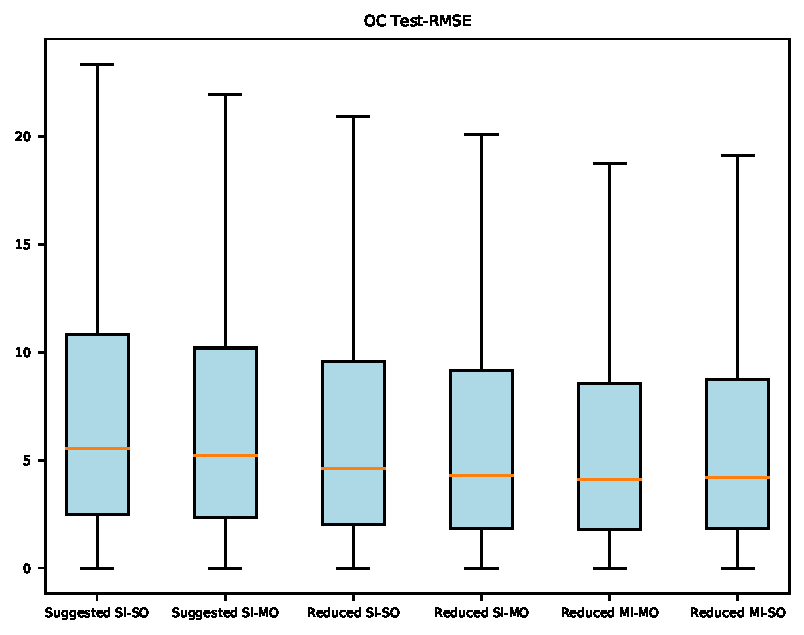
\includegraphics[width=1\linewidth]{RESULTS/BOXPLOTS/OC.pdf}
        \caption{Σύγκριση μοντέλων για την ιδιότητα του οργανικού άνθρακα}
        \label{fig:subim1}
    \end{subfigure}
    \begin{subfigure}{0.5\textwidth}
        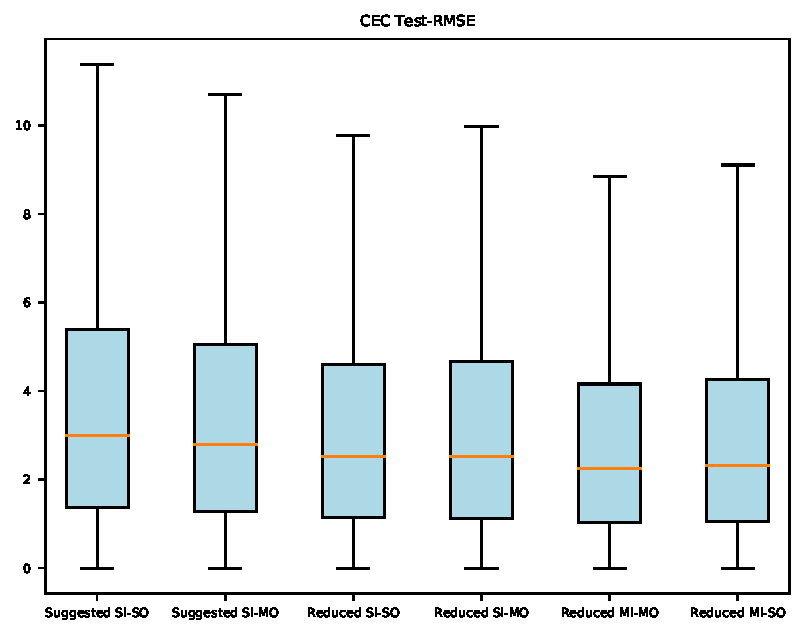
\includegraphics[width=1\linewidth]{RESULTS/BOXPLOTS/CEC.pdf}
        \caption{Σύγκριση μοντέλων για την ιδιότητα της ικανότητας ανταλλαγής κατιόντων}
        \label{fig:subim2}
    \end{subfigure}
\end{figure}
\begin{figure}[H]
    \begin{subfigure}{0.5\textwidth}
        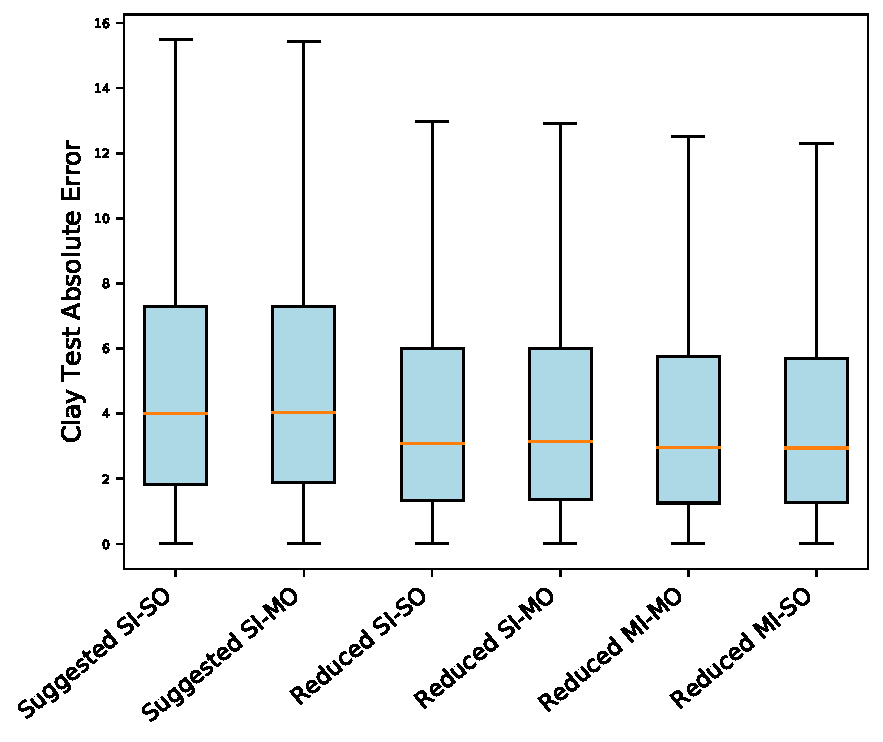
\includegraphics[width=1\linewidth]{RESULTS/BOXPLOTS/Clay.pdf}
        \caption{Σύγκριση μοντέλων για την ιδιότητα την περιεκτικότητα σε άργιλο}
        \label{fig:subim3}
    \end{subfigure}
    \begin{subfigure}{0.5\textwidth}
        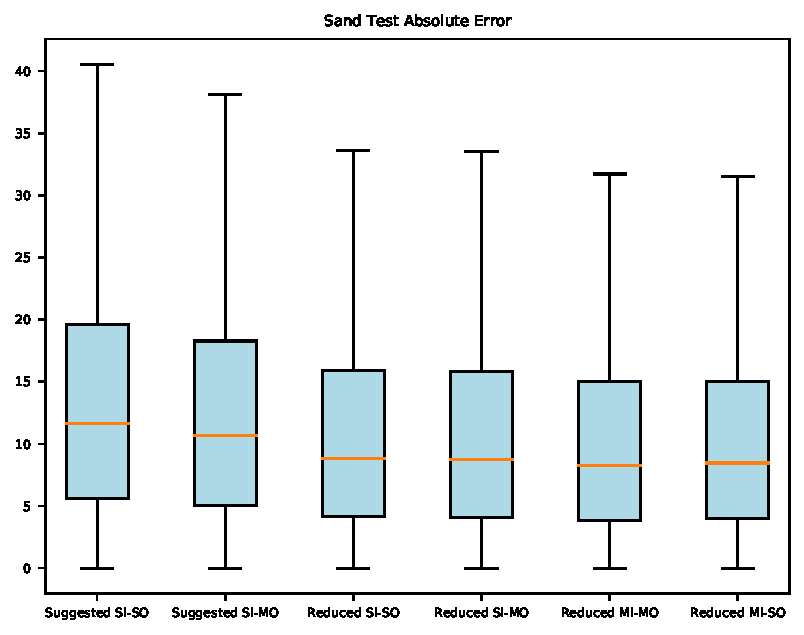
\includegraphics[width=1\linewidth]{RESULTS/BOXPLOTS/Sand.pdf}
        \caption{Σύγκριση μοντέλων για την ιδιότητα την περιεκτικότητα σε άμμο}
        \label{fig:subim4}
    \end{subfigure}
\end{figure}
\begin{figure}[H]
    \begin{subfigure}{0.5\textwidth}
        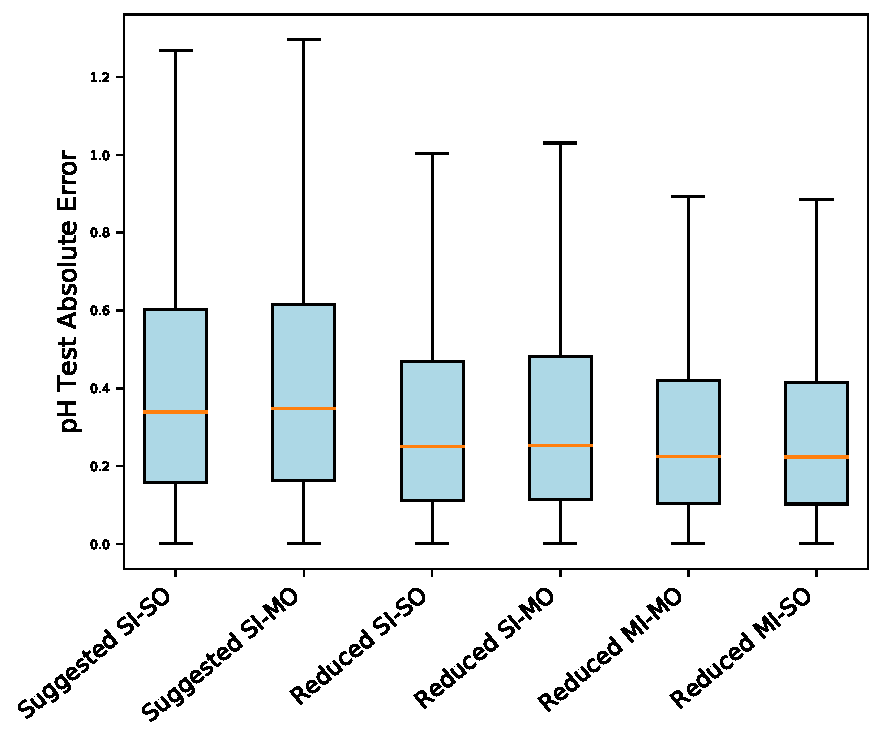
\includegraphics[width=1\linewidth]{RESULTS/BOXPLOTS/pH.pdf}
        \caption{Σύγκριση μοντέλων για την ιδιότητα την περιεκτικότητα του \tl{pH} στο νερό}
        \label{fig:subim5}
    \end{subfigure}
    \begin{subfigure}{0.5\textwidth}
        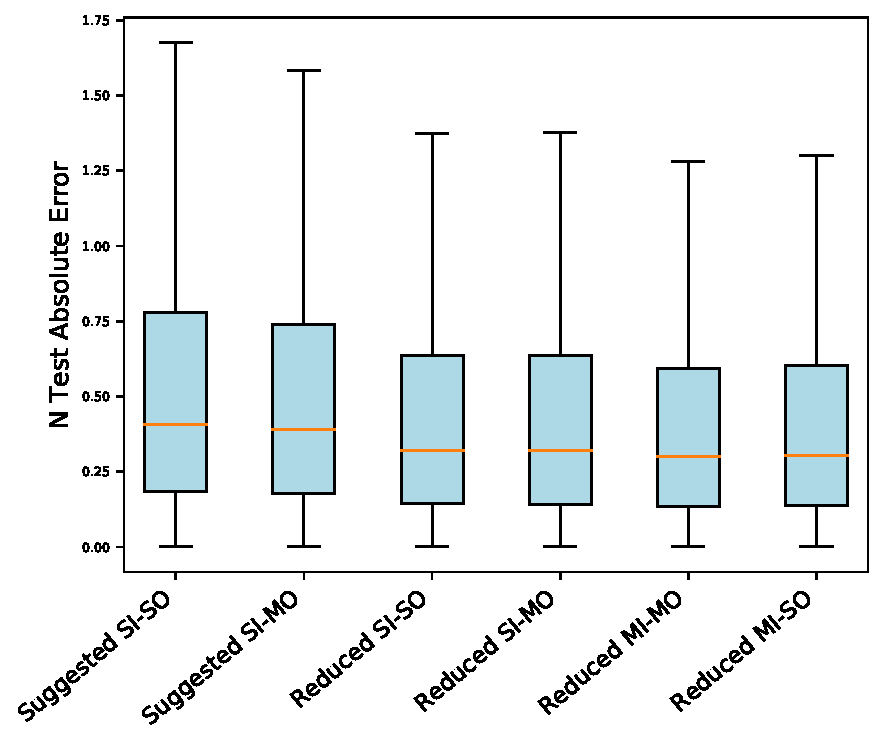
\includegraphics[width=1\linewidth]{RESULTS/BOXPLOTS/N.pdf}
        \caption{Σύγκριση μοντέλων για την ιδιότητα της περιεκτικότητας του αζώτου στο έδαφος}
        \label{fig:subim6}
    \end{subfigure}
\end{figure}
\begin{figure}[H]
    \begin{subfigure}{0.5\textwidth}
        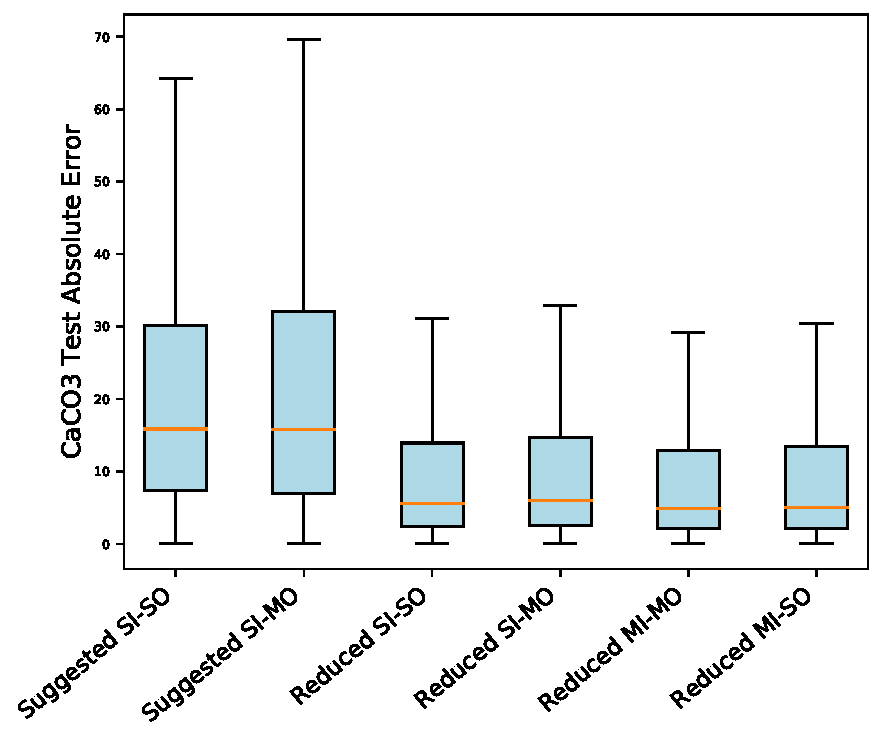
\includegraphics[width=1\linewidth]{RESULTS/BOXPLOTS/CaCO3.pdf}
        \caption{Σύγκριση μοντέλων για την ιδιότητα την περιεκτικότητα ανθρακικού ασβεστίου στο έδαφος}
        \label{fig:subim7}
    \end{subfigure}
    \begin{subfigure}{0.5\textwidth}
        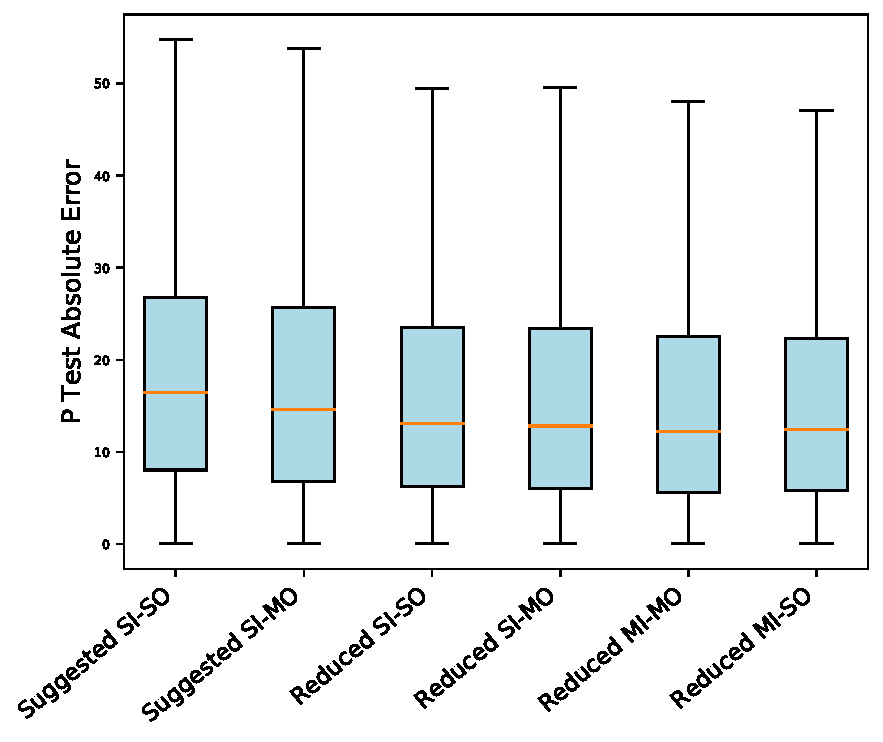
\includegraphics[width=1\linewidth]{RESULTS/BOXPLOTS/P.pdf}
        \caption{Σύγκριση μοντέλων για την ιδιότητα της περιεκτικότητας του φωσφόρου στο έδαφος}
        \label{fig:subim8}
    \end{subfigure}
\end{figure}
\begin{figure}[H]
    \begin{subfigure}{0.5\textwidth}
        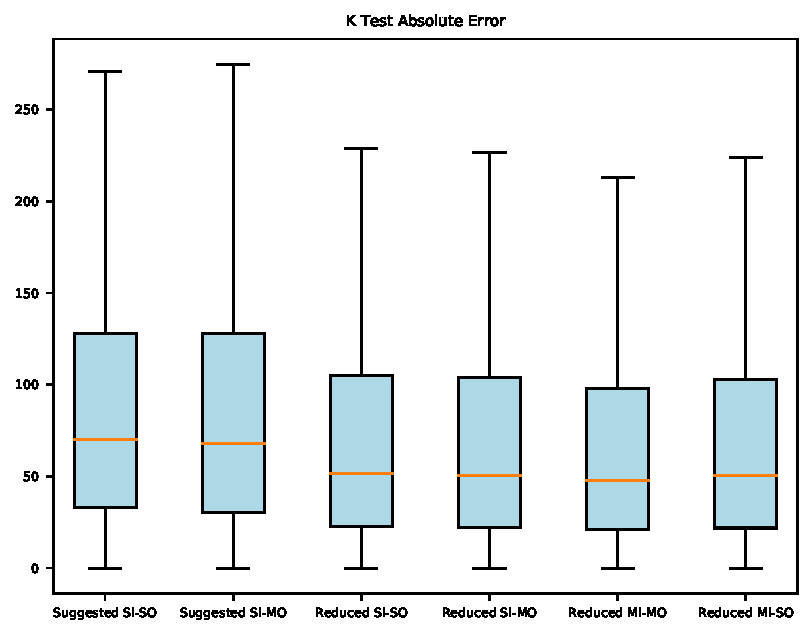
\includegraphics[width=1\linewidth]{RESULTS/BOXPLOTS/K.pdf}
        \caption{Σύγκριση μοντέλων για την ιδιότητα την περιεκτικότητα του καλίου στο έδαφος}
        \label{fig:subim9}
    \end{subfigure}
    \begin{subfigure}{0.5\textwidth}
        
    \end{subfigure}
\end{figure}

\begin{figure}[H]
    \begin{subfigure}{0.5\textwidth}
        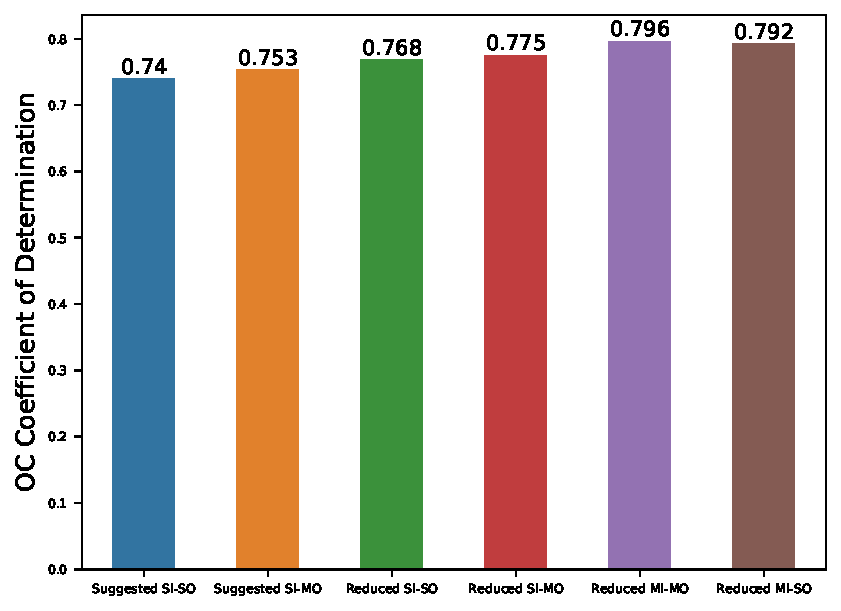
\includegraphics[width=1\linewidth]{RESULTS/BARPLOTS/test_OC_determ.pdf}
        \caption{Σύγκριση μοντέλων για την ιδιότητα του οργανικού άνθρακα}
        \label{fig:subim1}
    \end{subfigure}
    \begin{subfigure}{0.5\textwidth}
        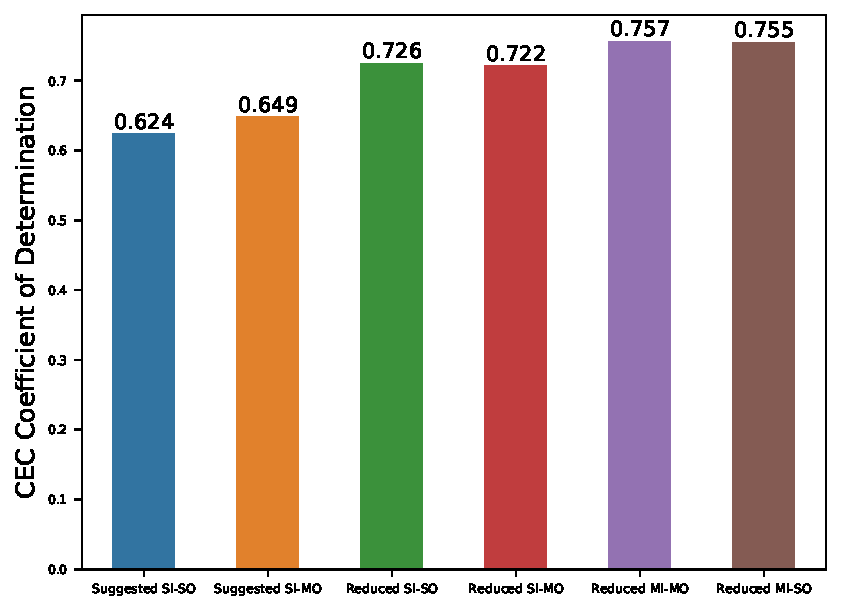
\includegraphics[width=1\linewidth]{RESULTS/BARPLOTS/test_CEC_determ.pdf}
        \caption{Σύγκριση μοντέλων για την ιδιότητα της ικανότητας ανταλλαγής κατιόντων}
        \label{fig:subim2}
    \end{subfigure}
\end{figure}
\begin{figure}[H]
    \begin{subfigure}{0.5\textwidth}
        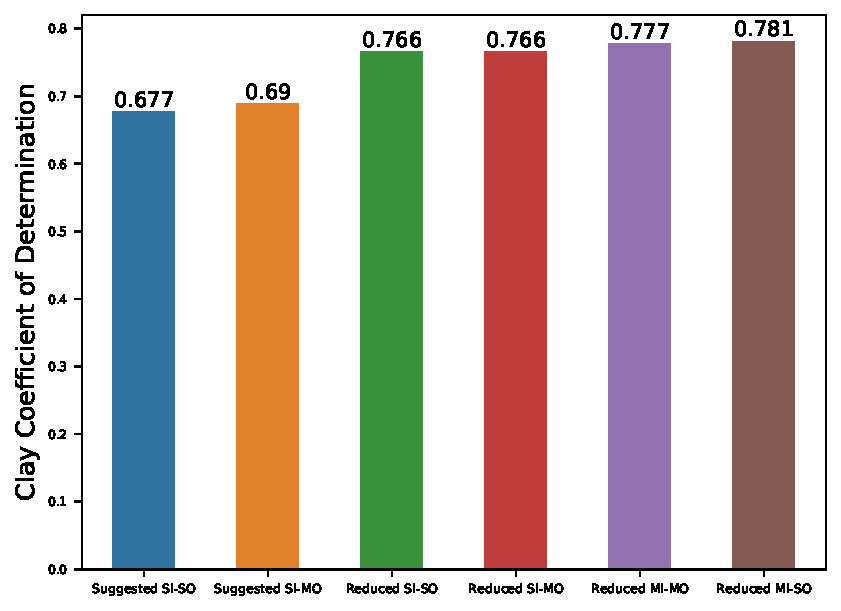
\includegraphics[width=1\linewidth]{RESULTS/BARPLOTS/test_Clay_determ.pdf}
        \caption{Σύγκριση μοντέλων για την ιδιότητα την περιεκτικότητα σε άργιλο}
        \label{fig:subim3}
    \end{subfigure}
    \begin{subfigure}{0.5\textwidth}
        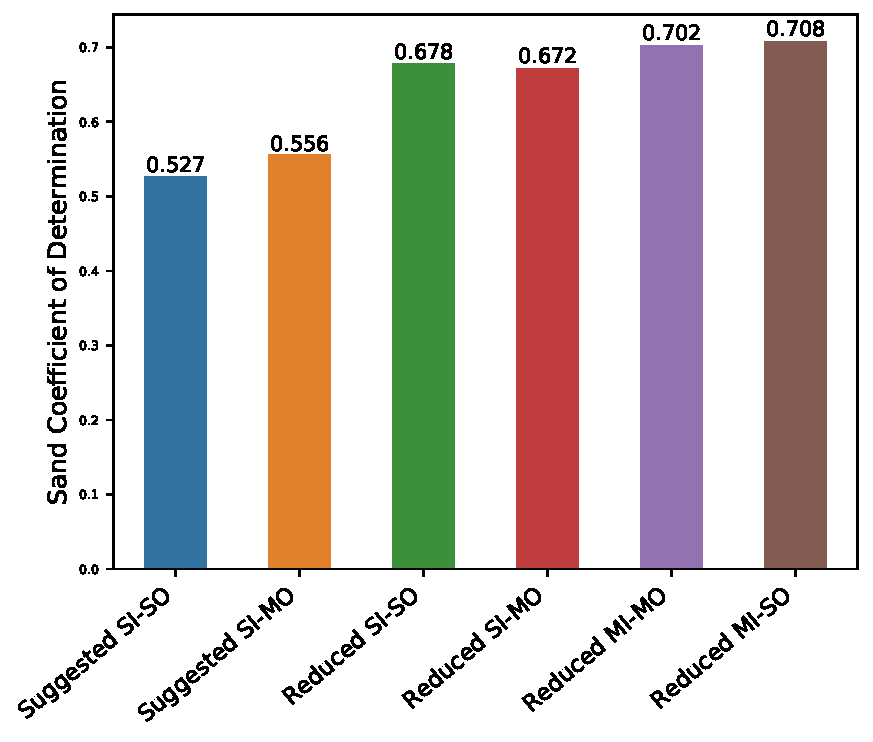
\includegraphics[width=1\linewidth]{RESULTS/BARPLOTS/test_Sand_determ.pdf}
        \caption{Σύγκριση μοντέλων για την ιδιότητα την περιεκτικότητα σε άμμο}
        \label{fig:subim4}
    \end{subfigure}
\end{figure}
\begin{figure}[H]
    \begin{subfigure}{0.5\textwidth}
        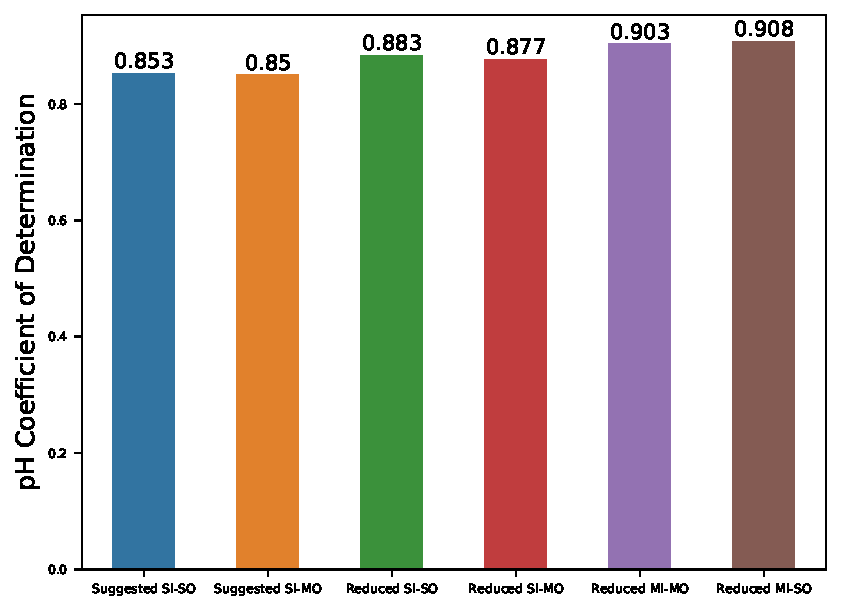
\includegraphics[width=1\linewidth]{RESULTS/BARPLOTS/test_pH_determ.pdf}
        \caption{Σύγκριση μοντέλων για την ιδιότητα την περιεκτικότητα του \tl{pH} στο νερό}
        \label{fig:subim5}
    \end{subfigure}
    \begin{subfigure}{0.5\textwidth}
        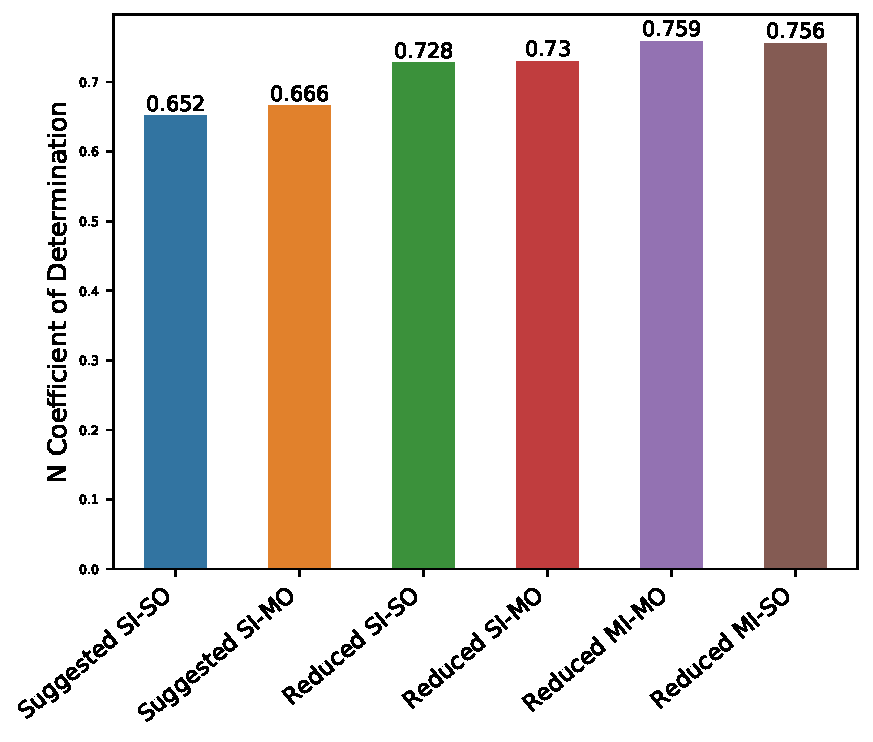
\includegraphics[width=1\linewidth]{RESULTS/BARPLOTS/test_N_determ.pdf}
        \caption{Σύγκριση μοντέλων για την ιδιότητα της περιεκτικότητας του αζώτου στο έδαφος}
        \label{fig:subim6}
    \end{subfigure}
\end{figure}
\begin{figure}[H]
    \begin{subfigure}{0.5\textwidth}
        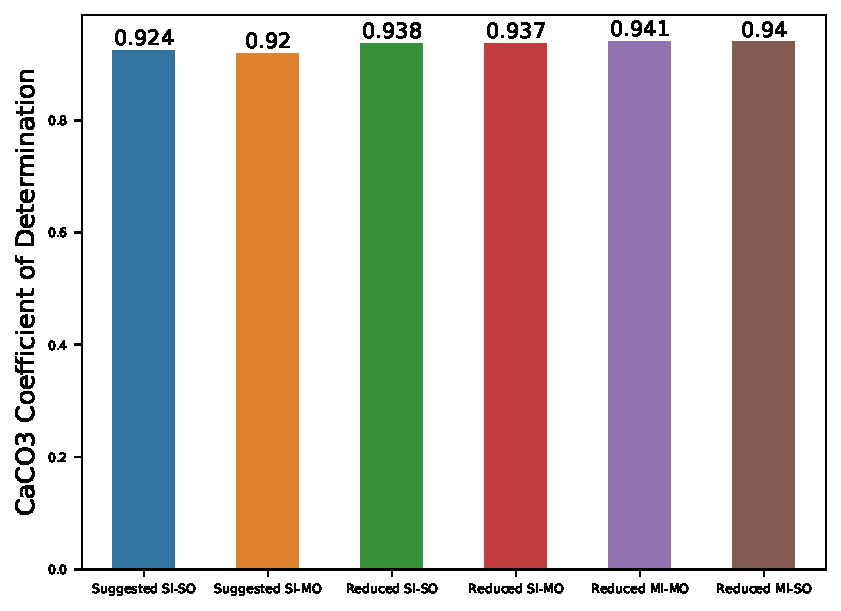
\includegraphics[width=1\linewidth]{RESULTS/BARPLOTS/test_CaCO3_determ.pdf}
        \caption{Σύγκριση μοντέλων για την ιδιότητα την περιεκτικότητα ανθρακικού ασβεστίου στο έδαφος}
        \label{fig:subim7}
    \end{subfigure}
    \begin{subfigure}{0.5\textwidth}
        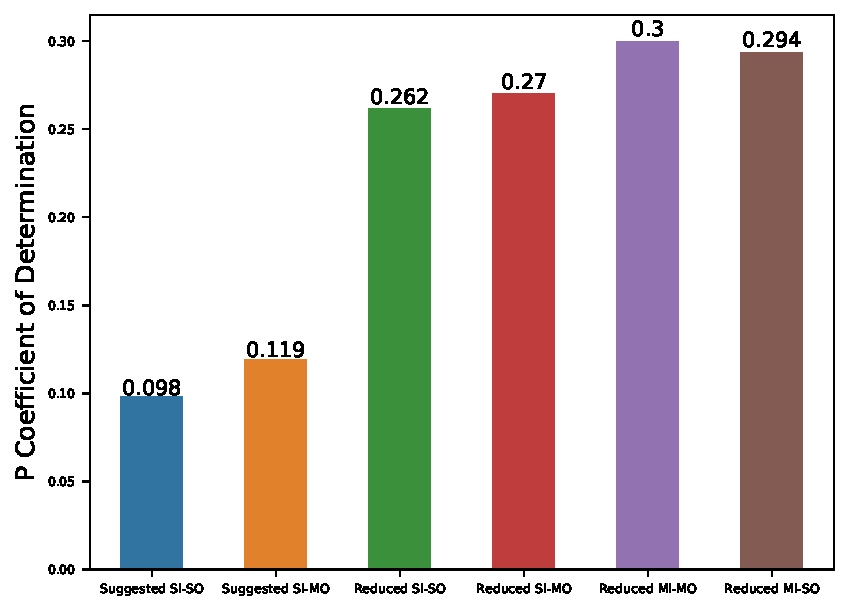
\includegraphics[width=1\linewidth]{RESULTS/BARPLOTS/test_P_determ.pdf}
        \caption{Σύγκριση μοντέλων για την ιδιότητα της περιεκτικότητας του φωσφόρου στο έδαφος}
        \label{fig:subim8}
    \end{subfigure}
\end{figure}
\begin{figure}[H]
    \begin{subfigure}{0.5\textwidth}
        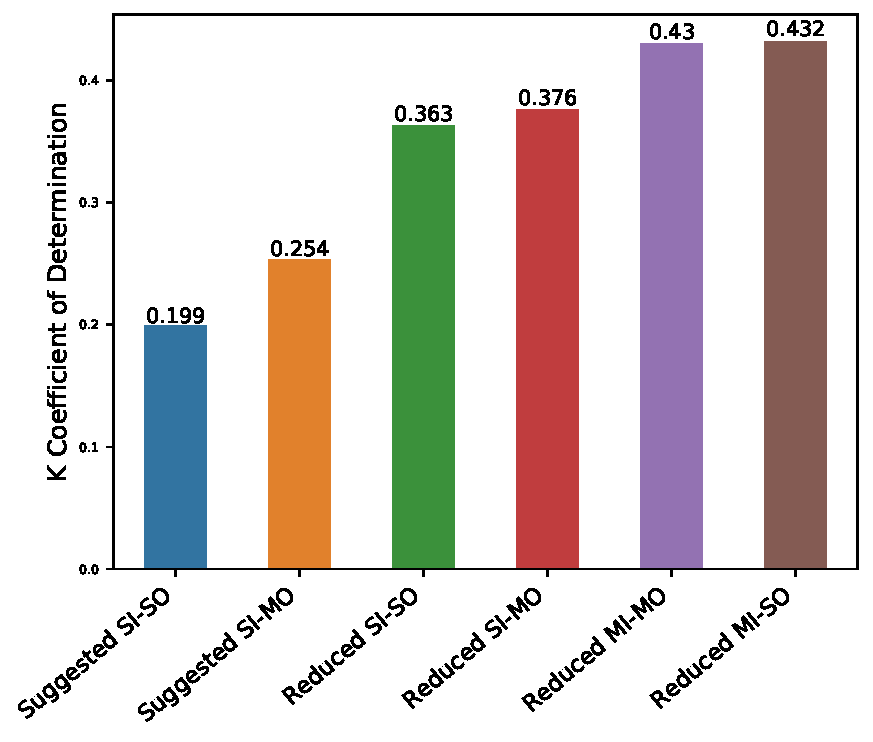
\includegraphics[width=1\linewidth]{RESULTS/BARPLOTS/test_K_determ.pdf}
        \caption{Σύγκριση μοντέλων για την ιδιότητα την περιεκτικότητα του καλίου στο έδαφος}
        \label{fig:subim9}
    \end{subfigure}
    \begin{subfigure}{0.5\textwidth}
        
    \end{subfigure}
\end{figure}

\section{Επιρροή του λόγου οριζόντιας προς κατακόρυφης διάστασης --- ανώτατο όριο αύξησης}
Η παράμετρος που ορίζει τον λόγο τον διαστάσεων της εικόνας εισόδου κατά την μετατροπή της φασματικής υπογραφή σε σπεκτρόγραμμα, παρατηρήθηκε πως επηρεάζει καθοριστικά την επίδοση των υλοποιήσεων δισδιάστατων συνελικτικών νευρωνικών δικτύων.\\
Για την εύρεση της βέλτιστης τιμής της παραμέτρου V/H Ratio χρησιμοποιήθηκε ένα μοντέλο πολλαπλών εισόδων και πολλαπλών εξόδων για την πρόβλεψη των περισσοτέρων ιδιοτήτων

\begin{figure}[H]
  \begin{center}
    \includesvg[width=1\textwidth]{RESULTS/Determ_v_h}
    \caption{Απόδοση του μοντέλου με βάση την μετρική $R^2$ συναρτήσει του λόγου κάθετης προς οριζόντιου διάστασης}
  \end{center}
\end{figure}

Όπως φαίνεται στο παραπάνω διάγραμμα, όταν η παράμετρος που ορίζει τον λόγο των διαστάσεων της εικόνας εισόδου, είναι στο εύρος τιμών 0.77 με 0.8 οι επιδόσεις του μοντέλου είναι κατά μέσο όρο μεγαλύτερες. Έτσι η τμή που επιλέχθηκε για τη συγκεκριμένη παράμετρο είναι το 0.8 καθώς παρουσιάζει την μέγιστη μέση επίδοση για τον συντελεστή προσδιορισμού όλων των εδαφικών ιδιοτήτων.

\section{Μείωση πλήθους \tl{Layers}}
Ένας από τους λόγους για τους οποίους η αρχιτεκτονική του μοντέλου των \tl{Padarian J. et al} θεωρείται μη αποτελεσματική είναι ότι χρησιμοποιεί μεγάλο πλήθος επιπέδων. Πέρα από την επιρροή του αριθμού των επιπέδων στο μέγεθός των παραμέτρων του μοντέλου, η συγκεκριμένη αποτελεί μια παράμετρο η οποία δοκιμάστηκε σε διάφορες μορφές της μέσα στην αρχιτεκτονική του δισδιάστατου συνελικτικού νευρωνικού δικτύου όπως στο πλήθος των συνελικτικών επιπέδων που χρησιμοποιούνται ή το πλήθος των πλήρων συνδεδεμένων επιπέδων\\

\textit{Παραδείγματα Αρχιτεκτονικών και Επιδόσεων}\\



\section{Επιρροή χρήσης \tl{Max Pooling}}
Όπως αναφέρθηκε στην θεωρητική ανάλυση των δισδιάστατων νευρωνικών δικτύων, τα επίπεδα συγκέντρωσης είναι από τα βασικά της συγκεκριμένης κατηγορίας μοντέλων. Ωστόσο εξετάστηκε η επίδραση της μείωσης του αριθμού των επιπέδων συγκέντρωσης, καθώς σε ορισμένες αρχιτεκτονικές του δοκιμάστηκαν έχουν μειωμένο αριθμό συνελικτικών επιπέδων. Κατά την δοκιμή της χρήσης διαφόρων αριθμών επιπέδων συγκέντρωσης παρατηρήθηκε πως η αφαίρεση όλων των επιπέδων συγκέντρωσης είχε ως αποτέλεσμα την σημαντική μείωση της επίδοσης του μοντέλου. Τελικά διαπιστώθηκε πως η βέλτιστη επίδοση του μοντέλου επιτυγχάνεται με χρήση ενός επιπέδου συγκέντρωσης.

Πίνακες επίδοσης μοντέλων με διάφορες χρήσεις επιπέδων συγκέντρωσης

Η συγκεκριμένη παράμετρος μπορεί να επηρεάσει σε μεγάλο βαθμό το συνολικό μέγεθος του μοντέλου, για παράδειγμα η αφαίρεση του επιπέδου συγκέντρωσης μεγίστων από το τελικό βέλτιστο μοντέλο

\section{Οπτικοποίηση συνελικτικών φίλτρων του μοντέλου}
Η φύση των δισδιάστατων νευρωνικών δικτύων τα καθιστά κατάλληλα για πειραματισμούς σχετικά με την μορφή της εισόδου που εισέρχεται στο μοντέλο σε κάθε επίπεδο του. Σε κάποιες περιπτώσεις οι μορφές των συνελικτικών φίλτρων θα μπορούσαν να ερμηνευτούν αναλόγως με τα χαρακτηριστικά που αφορούν την μορφή της εισόδου και την πληροφορία που αποσκοπείται να εξαχθεί από αυτή. Στην περίπτωση της εισόδου των μοντέλων που πραγματεύεται η παρούσα διπλωματική εργασία, τα μοτίβα που ανιχνεύονται στα σπεκτρογράμματα είναι ίσως κάποιες συγκεκριμένες διακυμάνσεις στις φασματικές υπογραφές και στους μετασχηματισμούς \tl{wavelet}.

Για την οπτικοποίηση των ενεργοποιήσεων των διαφόρων επιπέδων του μοντέλου εκπαιδεύεται ένα μοντέλο μιας εισόδου και μιας εξόδου, συγκεκριμένα  με τη χρήση φασματικών υπογραφών ανακλαστικότητας και με έξοδο την περιεκτικότητα σε οργανικό άνθρακα. Στη συνέχεια παρατίθενται οι μορφές των εξόδων κάθε επιπέδου από την είσοδο μέχρι το σημείο του μοντέλου όπου τα δεδομένα είναι σε δισδιάστατη μορφή.
\textit{Διαγραμμάτα}
\begin{figure}[H]
  \begin{center}
    \includesvg[width=1\textwidth]{RESULTS/model_layer_0_OC_input_3}
    \caption{Είσοδος μετά την μετατροπή σε σπεκτρόγραμμα από φασματική υπογραφή ανακλαστικότητας}
  \end{center}
\end{figure}

%\begin{figure}[htbp]
%    \begin{subfigure}{0.5\textwidth}
        %\includesvg[width=1\linewidth]{RESULTS/model_layer_1_OC_conv2d_4}
        %\caption{Πραγματικές τιμές}
        %\label{fig:subim1}
%    \end{subfigure}
%    \begin{subfigure}{0.5\textwidth}
        %\includesvg[width=1\linewidth]{RESULTS/model_layer_1_OC_conv2d_4_standarized}
        %\caption{Κανονικοποιημένες τιμές}
        %\label{fig:subim1}
%    \end{subfigure}
%    \caption{Μορφή της εξόδου του πρώτου δισδιάστατου συνελικτικού επιπέδου. Έξοδος για τα πρώτα 18 \tl{Feature %Maps}}
%\end{figure}
%
%\begin{figure}[H]
%  \begin{center}
%    \includesvg[width=0.3\textwidth]{RESULTS/model_layer_1_OC_conv2d_4_kernels}
%    \caption{Μορφή των συνελικιτκών φίλτρων που χρησιμοποιήθηκαν από το πρώτο δισδιάστατο συνελικτικό επιπέδο. %Φαίνονται τα  18 πρώτα φίλτρα}
%  \end{center}
%\end{figure}

\begin{figure}[htbp]
    \begin{subfigure}{0.7\textwidth}
        \begin{subfigure}{\textwidth}
            \includesvg[width=1\linewidth]{RESULTS/model_layer_1_OC_conv2d_4}
            \caption{Πραγματικές τιμές}
            \label{fig:subim1}
        \end{subfigure}
        \begin{subfigure}{\textwidth}
            \includesvg[width=1\linewidth]{RESULTS/model_layer_1_OC_conv2d_4_standarized}
            \caption{Κανονικοποιημένες τιμές}
            \label{fig:subim1}
        \end{subfigure}
    \end{subfigure}
    \begin{subfigure}{0.3\textwidth}
        \includesvg[width=\textwidth]{RESULTS/model_layer_1_OC_conv2d_4_kernels}
        \caption{Μορφή των συνελικιτκών φίλτρων που χρησιμοποιήθηκαν από το πρώτο δισδιάστατο συνελικτικό επιπέδο. Φαίνονται τα  18 πρώτα φίλτρα}
    \end{subfigure}
    \caption{Μορφή της εξόδου του πρώτου δισδιάστατου συνελικτικού επιπέδου. Έξοδος για τα πρώτα 18 \tl{Feature Maps}}
\end{figure}

\begin{figure}[htbp]
    \begin{subfigure}{0.5\textwidth}
        \includesvg[width=1\linewidth]{RESULTS/model_layer_2_OC_batch_normalization_8}
        \caption{Πραγματικές τιμές}
        \label{fig:subim1}
    \end{subfigure}
    \begin{subfigure}{0.5\textwidth}
        \includesvg[width=1\linewidth]{RESULTS/model_layer_2_OC_batch_normalization_8_standarized}
        \caption{Κανονικοποιημένες τιμές}
        \label{fig:subim2}
    \end{subfigure}
    \caption{Μορφή της εξόδου μετά το επίπεδο της κανονικοποίησης παρτίδας. Έξοδος για τα πρώτα 18 \tl{Feature Maps}}
\end{figure}

\begin{figure}[htbp]
    \begin{subfigure}{0.5\textwidth}
        \includesvg[width=1\linewidth]{RESULTS/model_layer_3_OC_re_lu_8}
        \caption{Πραγματικές τιμές}
        \label{fig:subim3}
    \end{subfigure}
    \begin{subfigure}{0.5\textwidth}
        \includesvg[width=1\linewidth]{RESULTS/model_layer_3_OC_re_lu_8_standarized}
        \caption{Κανονικοποιημένες τιμές}
        \label{fig:subim4}
    \end{subfigure}
    \caption{Μορφή της εξόδου του πρώτου δισδιάστατου συνελικτικού επιπέδου μετά την συνάρτηση ενεργοποίησης \tl{ReLU}. Έξοδος για τα πρώτα 18 \tl{Feature Maps}}
\end{figure}

\begin{figure}[htbp]
    \begin{subfigure}{0.5\textwidth}
        \includesvg[width=1\linewidth]{RESULTS/model_layer_4_OC_max_pooling2d_2}
        \caption{Πραγματικές τιμές}
        \label{fig:subim5}
    \end{subfigure}
    \begin{subfigure}{0.5\textwidth}
        \includesvg[width=1\linewidth]{RESULTS/model_layer_4_OC_max_pooling2d_2_standarized}
        \caption{Κανονικοποιημένες τιμές}
        \label{fig:subim6}
    \end{subfigure}
    \caption{Μορφή της εξόδου μετά την συνάρτηση ενεργοποίησης \tl{ReLU} του πρώτου επιπέδου και της εφαρμογής συγκέντρωσης μεγίστων. Έξοδος για τα πρώτα 18 \tl{Feature Maps}}
\end{figure}


\begin{figure}[htbp]
    \begin{subfigure}{0.7\textwidth}
        \begin{subfigure}{\textwidth}
            \includesvg[width=1\linewidth]{RESULTS/model_layer_5_OC_conv2d_5}
            \caption{Πραγματικές τιμές}
            \label{fig:subim1}
        \end{subfigure}
        \begin{subfigure}{\textwidth}
            \includesvg[width=1\linewidth]{RESULTS/model_layer_5_OC_conv2d_5_standarized}
            \caption{Κανονικοποιημένες τιμές}
            \label{fig:subim1}
        \end{subfigure}
    \end{subfigure}
    \begin{subfigure}{0.3\textwidth}
        \includesvg[width=\textwidth]{RESULTS/model_layer_5_OC_conv2d_5_kernels}
        \caption{Μορφή των συνελικιτκών φίλτρων που χρησιμοποιήθηκαν από το δεύτερο δισδιάστατο συνελικτικό επιπέδο. Φαίνονται τα  18 πρώτα φίλτρα}
    \end{subfigure}
    \caption{Μορφή της εξόδου του δευτερου δισδιάστατου συνελικτικού επιπέδου. Έξοδος για τα πρώτα 18 \tl{Feature Maps}}
\end{figure}

%\begin{figure}[htbp]
    %\begin{subfigure}{0.5\textwidth}
        %\includesvg[width=1\linewidth]{RESULTS/model_layer_5_OC_conv2d_5}
        %\caption{Πραγματικές τιμές}
        %\label{fig:subim7}
    %\end{subfigure}
    %\begin{subfigure}{0.5\textwidth}
        %\includesvg[width=1\linewidth]{RESULTS/model_layer_5_OC_conv2d_5_standarized}
        %\caption{Κανονικοποιημένες τιμές}
        %\label{fig:subim8}
    %\end{subfigure}
    %\caption{Μορφή της εξόδου του δευτερου δισδιάστατου συνελικτικού επιπέδου. Έξοδος για τα πρώτα 18 %\tl{Feature Maps}}
%\end{figure}
%
%\begin{figure}[H]
  %\begin{center}
%    \includesvg[width=0.3\textwidth]{RESULTS/model_layer_5_OC_conv2d_5_kernels}
%    \caption{Μορφή των συνελικιτκών φίλτρων που χρησιμοποιήθηκαν από το δεύτερο δισδιάστατο συνελικτικό επιπέδο. Φαίνονται τα  18 πρώτα φίλτρα}
  %\end{center}
%\end{figure}

\begin{figure}[htbp]
    \begin{subfigure}{0.5\textwidth}
        \includesvg[width=1\linewidth]{RESULTS/model_layer_6_OC_batch_normalization_9}
        \caption{Πραγματικές τιμές}
        \label{fig:subim9}
    \end{subfigure}
    \begin{subfigure}{0.5\textwidth}
        \includesvg[width=1\linewidth]{RESULTS/model_layer_6_OC_batch_normalization_9_standarized}
        \caption{Κανονικοποιημένες τιμές}
        \label{fig:subim10}
    \end{subfigure}
    \caption{Μορφή της εξόδου μετά το επίπεδο της κανονικοποίησης παρτίδας του δεύτερου συνελικτικού επιπέδου. Έξοδος για τα πρώτα 18 \tl{Feature Maps}}
\end{figure}

\begin{figure}[htbp]
    \begin{subfigure}{0.5\textwidth}
        \includesvg[width=1\linewidth]{RESULTS/model_layer_7_OC_re_lu_9}
        \caption{Πραγματικές τιμές}
        \label{fig:subim11}
    \end{subfigure}
    \begin{subfigure}{0.5\textwidth}
        \includesvg[width=1\linewidth]{RESULTS/model_layer_7_OC_re_lu_9_standarized}
        \caption{Κανονικοποιημένες τιμές}
        \label{fig:subim12}
    \end{subfigure}
    \caption{Μορφή της εξόδου του δεύτερου δισδιάστατου συνελικτικού επιπέδου μετά την συνάρτηση ενεργοποίησης \tl{ReLU}. Έξοδος για τα πρώτα 18 \tl{Feature Maps}}
\end{figure}

\textit{Σχολιασμοί για συνελικτικά επίπεδα, κανονικοποίηση παρτίδας, συνάρτηση ενεργοποίησης και επίπεδο συγκέντρωσης.}
Στις παραπάνω εικόνες φαίνεται ο τρόπος με τον οποίο ένα μοντέλο το οποίο έχει προηγουμένως εκπαιδευτεί, επεξεργάζεται την μονοκαναλική εικόνα εισόδου σε όλα τα επίπεδα τα οποία έχει δισδιάστατη μορφή. 